\documentclass{article}

\usepackage{microtype}
\usepackage{graphicx}
\usepackage{subfigure}
\usepackage{booktabs}
\usepackage{amsmath}
\usepackage{amsfonts}
\usepackage{dsfont}
\usepackage{float}
\usepackage{hyperref}
\usepackage{amssymb}
% \usepackage{icml2018}
\usepackage[accepted]{icml2018}

\icmltitlerunning{r1-arc-mini}

\begin{document}

\twocolumn[
  \icmltitle{Learning Curriculums for Abstract Reasoning on ARC-AGI}
  \centering
  \icmlauthor{Markus Zhang}{Stanford University}
  \icmlaffiliation{Stanford University}{Department of Computer Science}
  \icmlcorrespondingauthor{Markus Zhang}{markusz@stanford.edu}

  \vskip 0.3in
]

\printAffiliationsAndNotice{}

\begin{abstract}
  The benchmark ARC-AGI-1 has rule-based correctness rewards--suitable for DeepSeek-r1-series reasoning models. In this report we attempt to train an LLM policy capable of solving ARC-AGI puzzles via Group Relative Policy Optimization (GRPO) and curriculum learning. We evaluate bootstrapped baselines, including a small model fine-tuned on distilled reasoning traces, transduction- or induction-based outputs, and context length; we conclude that an untuned base model with DSL code generation is best. Then, we construct code sandboxes and DSL linters to shape rewards for both code correctness and style. Experiments show the hand-crafted reward curriculum successfully nudged the policy to output correct, executable DSL code. We observe slow unstable improvement on easy training puzzles, and unsucessful transfer to any evaluation puzzle within a 1-day 1xH100 compute budget.
\end{abstract}

\section{Motivation}
The ARC-AGI-1 \cite{ARC-AGI} benchmark has been saturated by compute-inefficient reasoning (o3) or test-time memorization (OmniARC) models \cite{openai_openai_nodate} \cite{OmniARC}. Recent reasoning models like DeepSeek-R1-Zero  have seen tremendous success in STEM reasoning by defining reward functions in tasks where the solution is provably correct or incorrect--for example, math questions by their numerical answers, and coding problems by their test cases. Puzzle attempts in ARC-AGI are also provably correct. In the \textit{transduction} case, where the model learns to explicitly output the guessed grid, the guess is either an exact match or not. In \textit{induction}, where the model learns to output a runnable function representing the guessed pattern, the function either yields the correct output for a given test input or not.

Framing ARC-AGI as a reasoning problem, we investigate whether the smaller reasoning model  can improve its baseline performance with Group Relative Policy Optimization \cite{GRPO}: sampling online trajectories in a group, estimating relative advantage, updating trust-region policy gradients.

ARC-AGI should be a \textit{narrow} reasoning task, in the sense that inputs and outputs grid shapes are well-defined and discrete, which implies that the number of abstract ideas that can be encoded in each puzzle should be relatively small. In contrast, many RL agents solve broad tasks, like independent browsing, where the ideal output is ill-defined. Therefore we hypothesized that a small model could learn to reason over these fixed patterns, but policy improvement was significantly slower and harder than exepcted, as will become clear.

\section{Related Work}



\paragraph{PPO} Proximal Policy Optimization \cite{PPO} belongs to a family of trust-region policy gradient methods. In a vanilla Policy Gradient,
\begin{align*}
  \mathcal{J}_{PG}(\theta) & = \mathbb{E}_{q \sim P(Q), o \sim \pi_\theta(O|q)}[A_{\pi_{\theta_{old}}}(q, o)]
\end{align*}
where $q,o$ are the question and output, and $A_{\pi_{\theta_{old}}}(q, o)$ is the advantage function typically estimated as $Q^{\pi_{\theta_{old}}}(q,o) - V^{\pi_{\theta_{old}}}(q)$. PPO adds a clipped surrogate objective to prevent destructively large policy updates:
\begin{align*}
  \mathcal{J}_{PPO}(\theta) & = \mathbb{E}_{q \sim P(Q), o \sim \pi_{\theta_{old}}(O|q)}\left[\min\left(r_\theta(q,o)A_{\pi_{\theta_{old}}}(q,o), \right.\right. \\
                            & \left.\left. \quad \text{clip}(r_\theta(q,o), 1-\varepsilon, 1+\varepsilon)A_{\pi_{\theta_{old}}}(q,o)\right)\right]
\end{align*}
where $r_\theta(q,o) = \frac{\pi_\theta(o|q)}{\pi_{\theta_{old}}(o|q)}$ is the probability action ratio between new and old policies, and $\varepsilon$ is a hyperparameter (typically 0.1 or 0.2) that bounds the policy change in a trust region, such that no single update pushes $r_\theta$ too far from 1.

\paragraph{GRPO} GRPO extends PPO by introducing group-relative advantages rather than critic-estimated advantages, introduced in the Approach section.

\paragraph{R1} The DeepSeek R1 series \cite{r1} builds from verification-based learning, starting with R1-Zero from V3 baseline on GRPO with rule-based rewards for math and code tasks. R1 then warm-starts from human-cleaned R1-Zero thought patterns or few-shot learning with extended chain-of-thought reasoning.

\paragraph{DSL} \cite{Hodel} constructed a domain-specific language with syntax, generator, and verifier functions specifically designed for ARC tasks. Their verifier automatically checks test-case outputs without requiring natural language explanations. While their DSL covers all 400 training and 400 public evaluation tasks, it potentially overfits to the training distribution since it was iteratively designed alongside task solvers.

\paragraph{Augmentation} Several efforts focus on expanding the limited ARC dataset. BARC \cite{barc} generated 400,000 ARC-Heavy remixed examples using GPT-4o, though only seed tasks were verified. The MIT approach \cite{MIT} leverages permutation transforms and in-context learning in a leave-one-out fashion, applying auxiliary losses on context grids. They create new LoRA adapters per test task to maximize performance. MindsAI's unpublished work, known primarily through reverse-engineering efforts, combines synthetic data from reARC with geometric transformations, followed by test-time fine-tuning.

\paragraph{Voting} OmniARC \cite{OmniARC} employs multiple surrogate approaches including traditional example-to-output mapping, code induction solving, input distribution learning, verification, and output selection through voting. Their workflow involves fine-tuning smaller models like Qwen-2.5-0.5B with LoRA, augmenting test sets, and applying ensemble voting. The MIT team uses two-round voting across geometric permutations and leave-one-out orderings.

\paragraph{Rejection Sampling} \cite{Greenblatt} used the GPT-4o API only with massively parallel rejection sampling and iterative healing (ask model to fix its own mistakes given code output) to achieve 50\% on ARC Public Eval. \cite{Jeremy} extended this with guided sampling via evolutionary algorithms that reproduce good reasoning strands that have high correct rates on the puzzle's in-context examples.

We borrow DSL work from \cite{Hodel} and GRPO from \cite{GRPO}, while other test-time scaling ideas do not obviously apply due to the different SFT / RL training settings.

\section{Initial Approach}

\subsection{Transduction}

Initially, our approach was not code generation but direct transduction. That is, we aimed to train the model to generate the direct $(m \times n)$ output grid rather than the Python DSL function that solves any given input grid. Given the significant performance gap between small models and larger reasoning models like R1, we sought to create a strong fine-tuned baseline.

Our first strategy involved bootstrapping a good policy by fine-tuning on the reasoning traces of larger models--a form of distillation found in s1 \cite{s1}. Verification was performed through rejection sampling, but this turned out to be highly inefficient. Even larger models struggled to solve most tasks, and increasing the number of rejections yielded diminishing returns.

\subsection{Reasoning Distillation}

We encountered a "blabbering" problem: teacher models like \texttt{DeepSeek-R1-Llama-70B} would produce excessively long reasoning traces that often overflowed the 32k context window. These traces frequently contained many incorrect approaches before potentially arriving at a correct conclusion. For example, one model persistently tried to count color numbers and sum them across rows—-a fundamentally flawed approach since operations like adding colors (e.g., green $=3$, blue $=2$, but green $+$ blue $\neq 5$) are not meaningful in the context of these puzzles. Even explicit prompting against such invalid operations failed to redirect the model's reasoning.

At 100 samples per puzzle, larger models still demonstrated difficulty, and increasing the magnitude of rejection sampling barely improved results. For $k$ distinct thought patterns in a reasoning trace separated by \texttt{\{Wait, Alternatively, But, ... \}}, often the $(k-1)$ patterns were incorrect, with only the last $1$ step. r1 would procrastinate, with a correct pattern appearing near the end of the model's context window, as documented in \cite{qu_optimizing_2025}. This indicates that unnecessarily long reasoning traces risk rewarding incorrect thought patterns since the rejection sampling rule is "final step correct".

As an alterative, we tried generating reasoning traces by prompting with a \texttt{(problem, solution)} pair--the key difference being that the solution is given. However, we observed test leakage in generated reasoning, where the model would reveal it already knows the answer. Such a training set can cause hallucination.

We also considered starting with easy-rated tasks via curriculum learning, allowing teacher models to generate more reliable reasoning traces for simpler problems. However, this raised questions about whether such selective SFT would provide a better prior than direct reinforcement learning.

For these all reasons and high API cost, accepted teacher samples were too sparse for distillation to be feasible, much less efficient. Therefore we attempted direct GRPO with an untuned HuggingFace baseline policy model.

\subsection{Induction}

Even without fine-tuning, we observed that reasoning models had a tendency to hallucinate incorrect reasoning patterns and verification steps, so we switched to inductive code generation. Instead of manually verifying correctness within in-context examples, we leveraged the model's latent coding ability from pretraining and distillation.

Inductive code generation provided the additional benefit of being executable on all in-context examples. If a program $\hat{f}$ was correct for the in-context examples $(x_i, y_i)_{i=1}^n$, such that $\hat{f}(x_i) = y_i$ for all $i$, then it is shown by \cite{Hodel} that for the test example, $\hat{f}(x_{n+1}) = y_{n+1}$. In other words, the puzzles have no ambiguity between the in-context and test examples.

Moreover, code execution shifts the policy $\pi$'s action space $\mathcal{A}$ from the set of all $(n \times m)$ grids to the set of all programs. Since we know the CommonCrawl pretraining has (GitHub, StackOverflow) code aplenty and fewer puzzles, we hypothesized that code generation would be a more natural transfer task for the base LLM, and therefore more sample efficient.

% In the future, the execution output can be a tool response to allow self-healing and end-to-end training with multi-tool calling.

\section{Final Approach}

\subsection{GRPO}

Following \cite{r1,GRPO}, we adopt Group Relative Policy Optimization (GRPO). For any question $q$ in the dataset, GRPO samples $G$ trajectories $\{o_i\}_{i=1}^G$ of output and reasoning traces. On the policy gradient step, we maximize the objective
\begin{align*}
   & \mathcal{J}_{GRPO}(\theta)  = \mathbb{E}_{q \sim P(Q), \{o_i\}_{i=1}^G \sim \pi_{\theta_{old}}(O \mid q)} \\
   & [ \frac{1}{G} \sum_{i=1}^G ( \min ( r_iA_i, clip(r_iA_i, 1-\varepsilon, 1+\varepsilon) )                  \\ & - \beta \mathbb{D}_{KL}(\pi_\theta \| \pi_{ref}) ) ]
\end{align*}
where $r_i$ is the action ratio, and advantage $A_i$ is estimated critic-free relative to the group's mean normalized rewards:
$$
  A_i = \frac{r_i - \operatorname{mean}(\{r_1, r_2, \ldots, r_G\})}{\operatorname{std}(\{r_1, r_2, \ldots, r_G\})}, \quad r_i = \frac{\pi_\theta(o_i \mid q)}{\pi_{\theta_{old}}(o_i \mid q)}
$$
instead of typical PPO advantage $A_i = Q^{\pi_{\theta_{old}}}(o_i, q) - V^{\pi_{\theta_{old}}}(q)$.

We train the baseline \texttt{DeepSeek-R1-Distill- Qwen-7B} with Unsloth \cite{unsloth}, a patch of HuggingFace TRL \cite{trl} optimized with single-GPU CUDA kernels. To run online GRPO, we alternate between sampling online off-policy trajectories on vLLM \cite{vllm} and updating gradients on TRL. It implies a significant memory overhead with a full cycle of model unload/load per batch, and lowers our MFU to 50\%, which is systems optimization left to future work.

\begin{figure}[t]
  \centering
  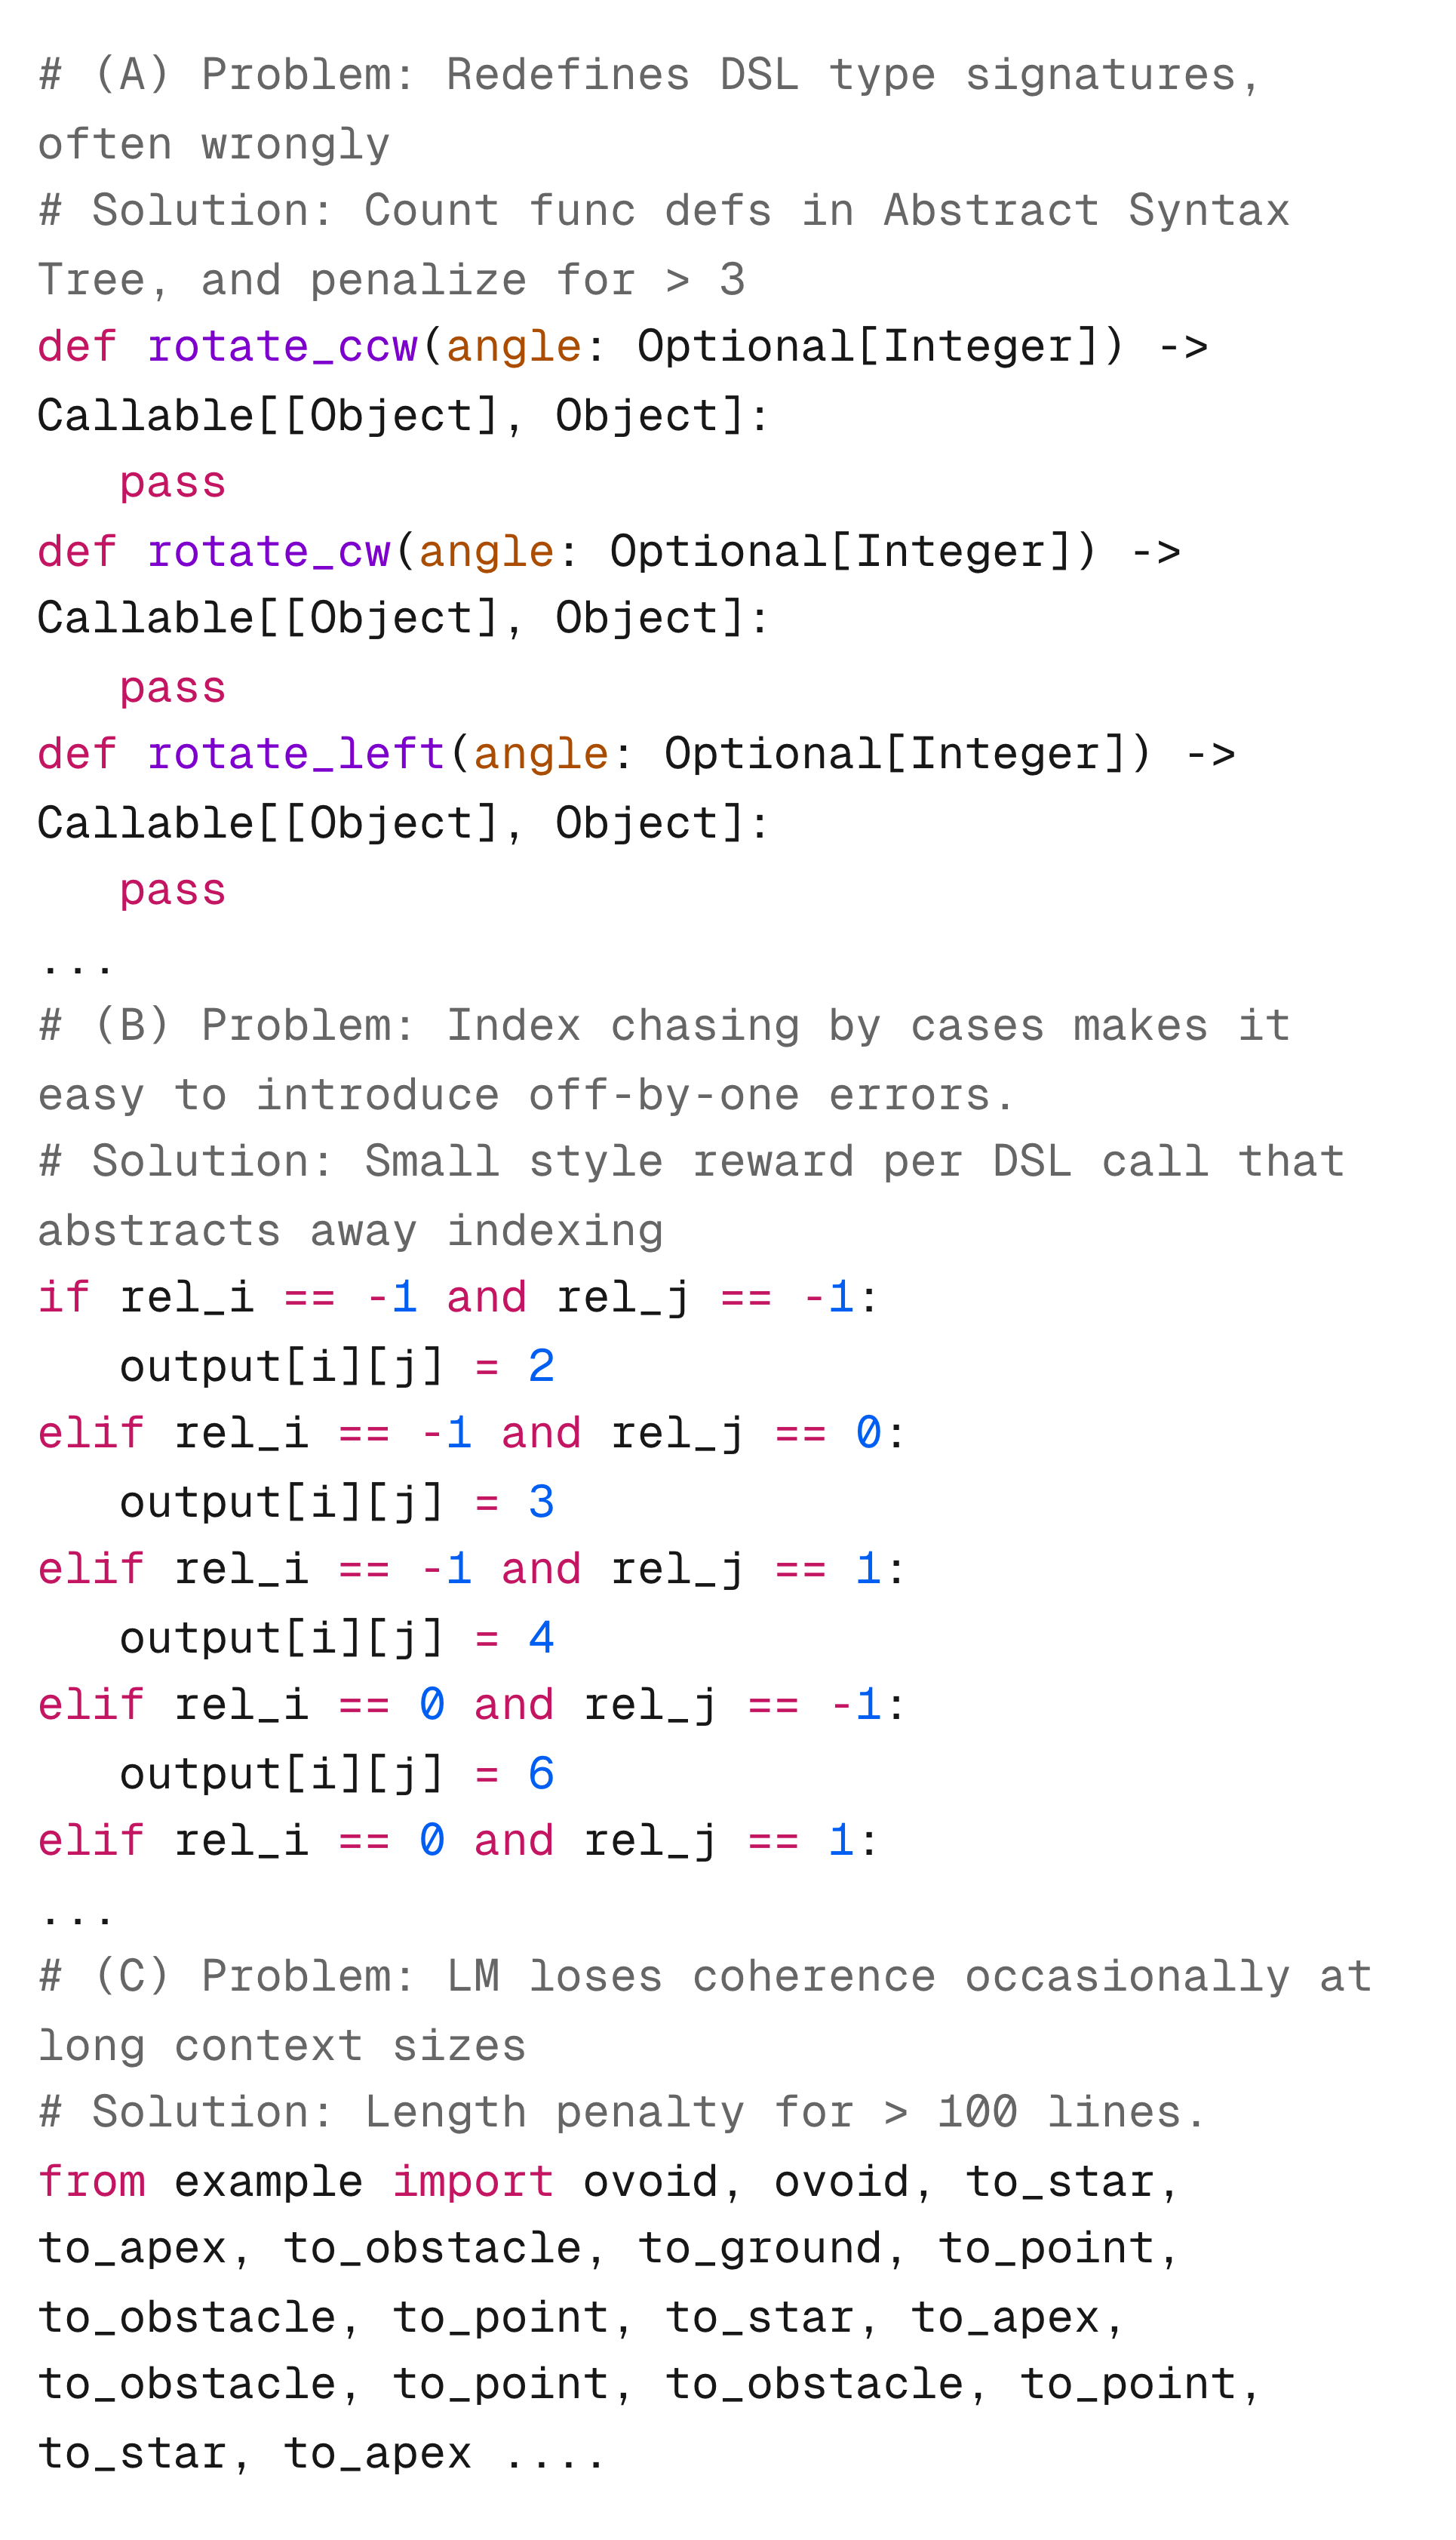
\includegraphics[width=0.5\textwidth]{bin/failures.png}
  \caption{Policy codegen failures, patched with reward shaping}
  \label{fig:failures}
\end{figure}

\subsection{DSL}

However, initial results showed that the policy model struggled primarily with index chasing—handling complex displacements within a puzzle grid (Figure \ref{fig:failures}B). Occasionally, the policy reasoned through the correct intuition but failed to implement it correctly in code. This flaw in reward function design led to correct reasoning gone unrewarded, if the output was wrong and the Code Interpreter returned \texttt{IndexError} or \texttt{KeyError}. Consequently, the advantage was low, and the model received zero reward despite showing partial correctness This flaw is common to Outcome Reward Modelling (ORM), but it is hard to implement an objective verifier for intermediate reasoning steps for Process Reward Modelling (PRM).

Instead we borrow ARC-DSL from \cite{Hodel} and nudge the policy to shift its output distribution, from any Python to a domain-specific language  implemented as a subset of Python. Since each pattern in ARC puzzles is a very simple geometric transformation (i.e. rotate shape, fill in color, find objects), it is intuitive that pure Python introduces needless complexity by index-chasing. It is simpler to define new ARC-DSL primitives available to the policy (i.e. \texttt{rot90(), fill(), objects()}). The $164$ DSL primitives are tested for correctness ahead-of-time, and their function signatures are loaded into every policy's prompt. ARC-DSL covers all $400$ training and $400$ public evaluation tasks, and it was iteratively designed alongside human-written puzzle solvers, prioritizing imperative functional syntax and minimal redundancy.

\subsection{Parsers, Linters, and CFGs}

The model showed initial reluctance to use our DSL, defaulting to deeply nested Python indexing notation or redundantly re-importing/defining DSL function definitions (Figure \ref{fig:failures}A). To counteract this, we added a style reward for using DSL functions correctly, and a style penalty for excessive function definitions.

To implement style penalties, we use Python's \texttt{ast, cst} parsers to construct Abstract and Concrete Syntax Trees of codegens. The static analysis enables counting of function definitions, calls, function length, and other metrics.


Although the policy eventually learned to use ARC-DSL through our reward signals, convergence was slow and took 12h on 1xH100. Therefore we wondered if we could improve sample-efficiency by implementing guided decoding to force each logit in the LM output to conform to the DSL format (Figure \ref{fig:dsl}). This is best expressed as a context-free grammar (CFG) of ARC-DSL, which restricts the next LM token to be in the expected set of lexer tokens. We implemented a CFG for \texttt{ARC-DSL} in Lark with a LALR(1) parser. Per the style of Figure \ref{fig:dsl}, is a small subset of the full Python CFG and restricts: all function definitions to have the name \texttt{solve()}; all variable names to be \texttt{x\{number\}}; every assign statement to be 1 pure DSL function call. While the CFG could successfully validate a static code snippet, streaming token-by-token input from the vLLM decoder created instabilities, where LALR could not parse partial code chunks. One bad CFG token read often crashed the training run, and the systems implementation effort to make \texttt{Lark -> vLLM -> TRL -> Unsloth} all mutually compatible was too high. Hence in our final training, we did not use guided decoding, but we believe this is a promising direction to allow faster policy improvement at the start; if code style has built-in enforcement, it does not need to be modelled as a separate reward, which reduces the risk of bad reward surrogates.

\begin{figure}[t]
  \subfigure{
    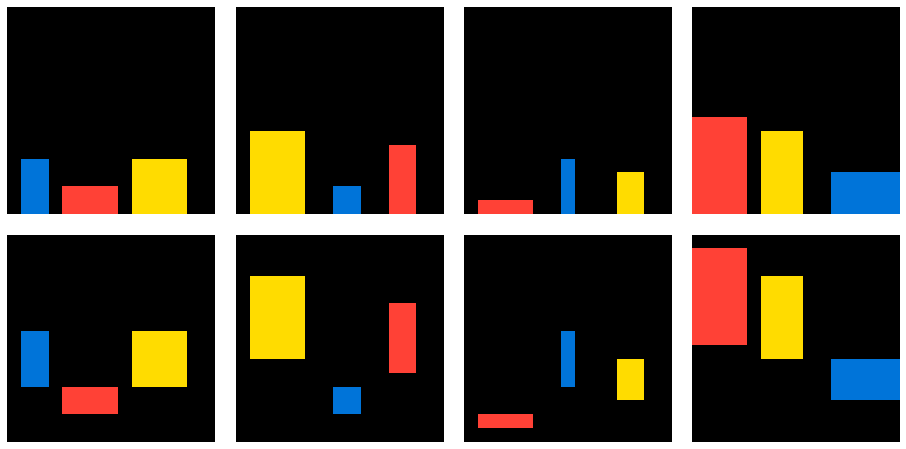
\includegraphics[width=0.95\columnwidth]{bin/5521c0d9.png}
  }
  \subfigure{
    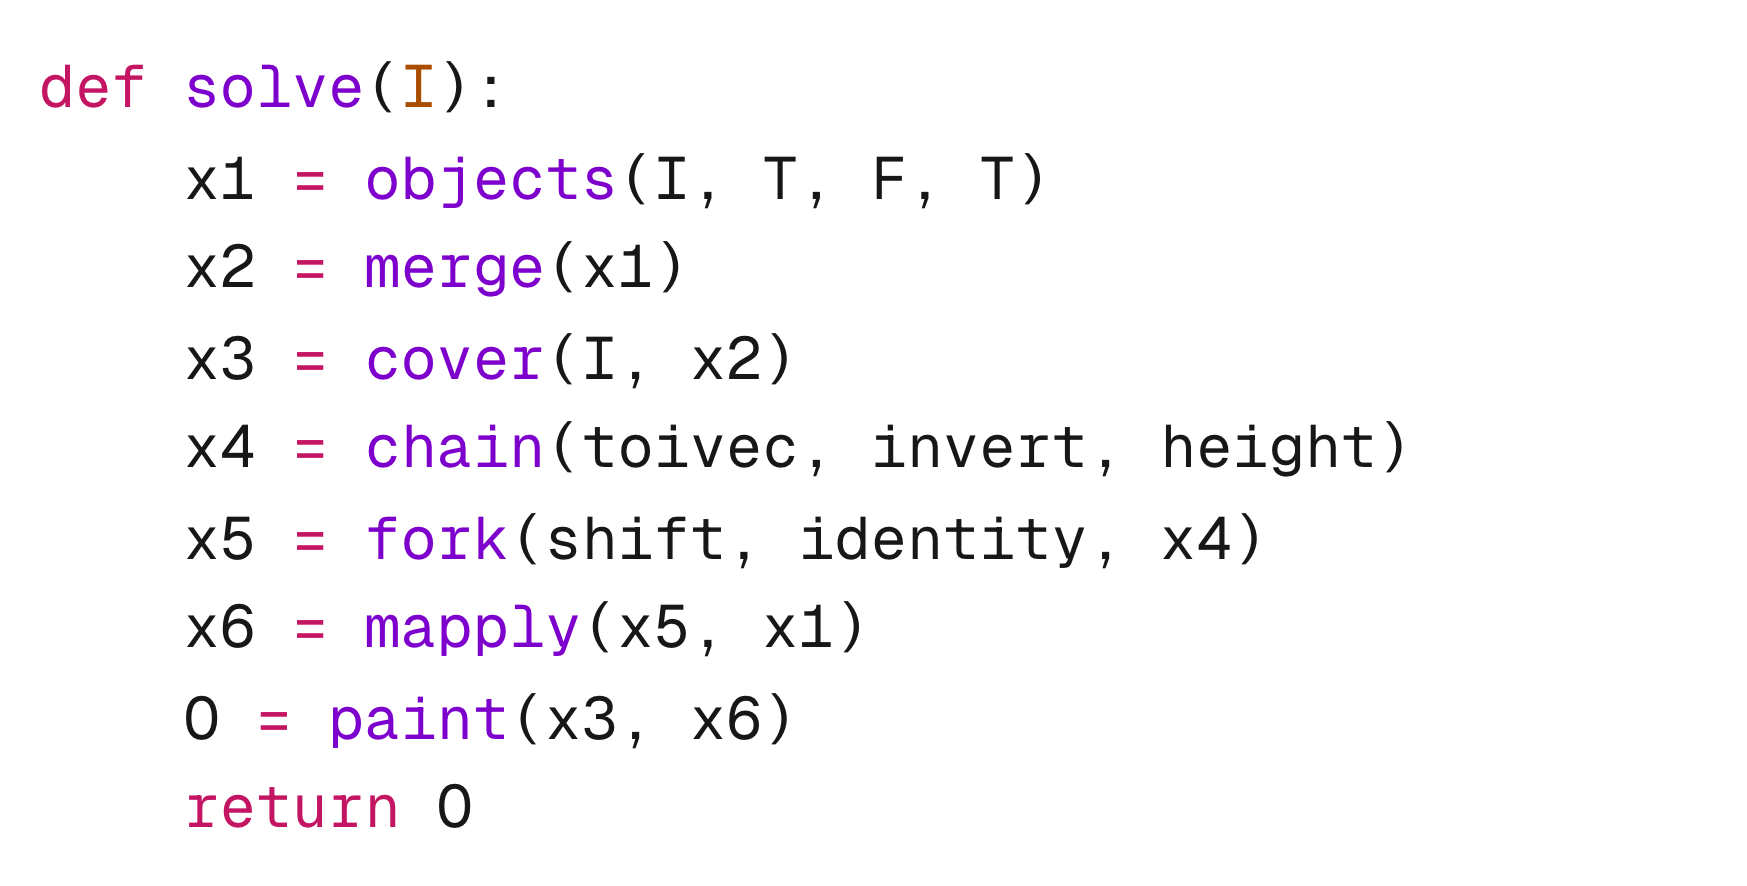
\includegraphics[width=0.95\columnwidth]{bin/solver_5521c0d9.png}
  }
  \caption{A Puzzle \texttt{5521c0d9} with the DSL solution. The rule is to levitate every colored box at a height defined the box's height.}
  \label{fig:dsl}
\end{figure}


\subsection{Execution Sandbox}

To ensure execution ran smoothly, we implemented an isolated execution sandbox in a \texttt{subprocess}, where arguments were passed in as command-line flags, and return values were piped to a JSON file. This was necessary to prevent reward hacking, where the model could exploit unintended behaviors by accessing networks or solution files. More importantly, any runtime error is fully contained in the sandbox, thereby preventing bad output code from taking down the whole training run.

Ensuring reliable code interpretation was a challenge. Initially, we added a tracer to track variable states and intermediate assignments, similar to a debugger. However, models frequently generated code that broke the placement of tracer hooks, such as forgetting \texttt{return}, deep function nesting, or infinite loops. Due to unreliable inspection of intermediate states, we ultimately decided to only inspect full function inputs and outputs.


\subsection{Reward Function}

The reward $r = r_{correct} + r_{style}$, defined as follows.
\paragraph{Soft Correctness} - We create finely graduated reward for more training stability. Before being correct ($r_{correct} = 1$), an output code must run ($runs$), must output the correct shape ($shape$), and have some ratio of grids correct ($r_{correct}$). The polynomial $r_{correct}^{5}$ amplifies the reward for the last-few wrong grid cells, and $n_o \in \{1,2\}$ is the number of puzzle test outputs.
$$
  \begin{aligned}
    r_{correct} & = 1.2\, \mathds{1} [runs] + \sum_{i=0}^{n_o} \left( 0.5\, \mathds{1} [shape] + r_{correct}^{5} \right)
  \end{aligned}
$$
\paragraph{Style} - Rewards correct syntax ($syntax$) and number of DSL functions used ($n_{dsl}$)--with $O(\sqrt{\cdot})$ growth to discourage reward hacking by spamming DSL calls. Also linear penalties for excessive function definitions ($n_{func}$), lines of code ($n_{lines}$).
$$
  \begin{aligned}
    r_{style} & = 0.1 \,\mathds{1} [syntax] + \sqrt{n_{dsl}} \\ &- 0.1 \, max(n_{func} - 3, 0) \\ &- 0.2 \, max(n_{lines} - 100, 0)
  \end{aligned}
$$

This design counters the increasing marginal effort required to reason correctly about additional correct cells in the grid, ensuring that late-stage improvements are still incentivized. The big intermediate rewards are to nudge the policy in the beginning when almost no puzzles are solved correctly, counteracting the sparse reward landscape at start.

\begin{figure*}[t]
  \centering
  \subfigure[Soft Correctness Reward. The policy only achieves run reward reliably around step 700.]{
    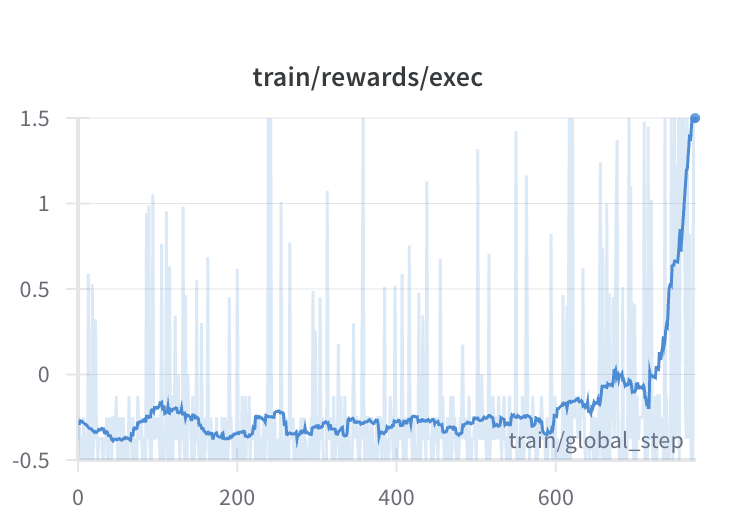
\includegraphics[width=0.95\columnwidth]{bin/exec.png}
    \label{fig:exec}
  }
  \hspace{0.05\columnwidth}
  \subfigure[Style Reward. The large penalties disappear early around step 700; after, the policy consistently earns DSL function call reward.]{
    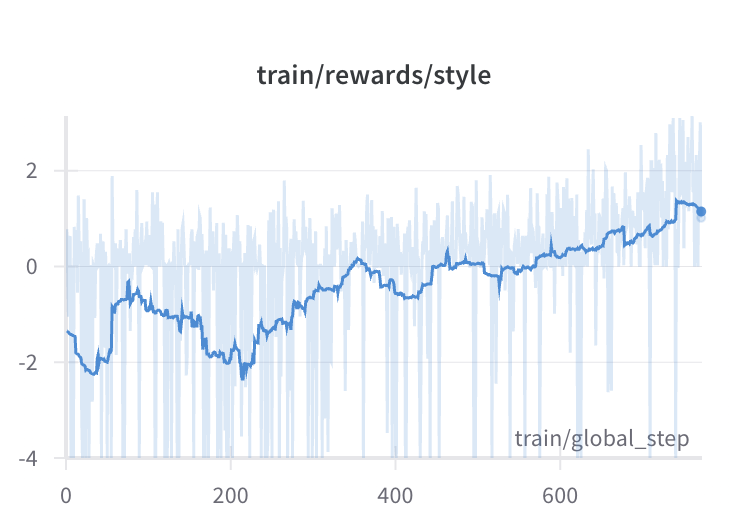
\includegraphics[width=0.95\columnwidth]{bin/style.png}
    \label{fig:style}
  }
  \subfigure[Total Reward. Curvature is dominated more by style than correctness, which may imply that (1) policy needs more compute beyond the training budget to improve more, or (2) the reward is misspecified.]{
    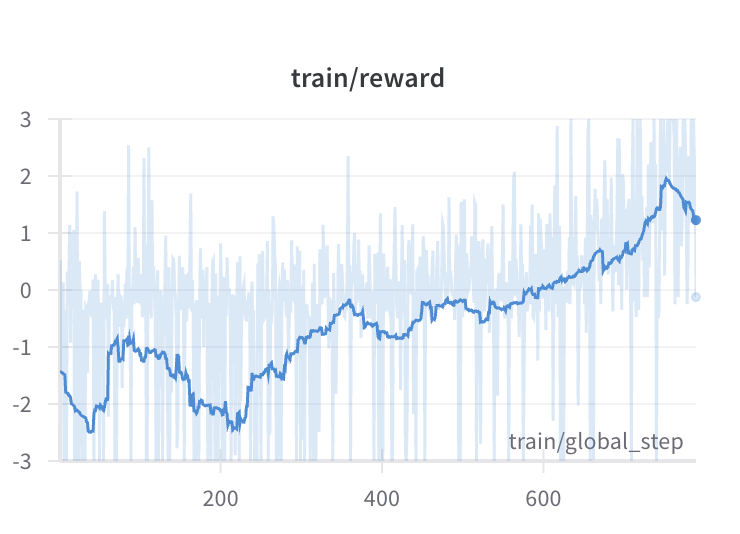
\includegraphics[width=0.95\columnwidth]{bin/reward.png}
    \label{fig:reward}
  }
  \hspace{0.05\columnwidth}
  \subfigure[Reasoning and Output Length. In a reversal of R1-Zero's 'aha' moment, this policy learns to think less. Likely, it learnt to 'blabber' less and discard earlier thought patterns.]{
    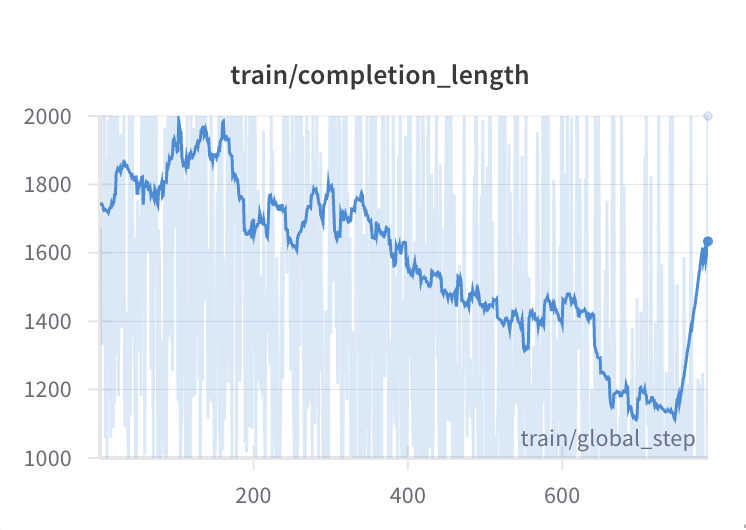
\includegraphics[width=0.95\columnwidth]{bin/length.png}
    \label{fig:length}
  }
  \caption{WandB plots for the final, longest training run of 1-day on 1xH100. vLLM online sampling slows training considerably.}
  \label{fig:grid2x2}
\end{figure*}

Since advantage $A_i$s are estimated in-group, large intermediate rewards do not create reward local maxima. For example, if all group outputs receive the runtime reward $1.2\, \mathds{1} [runs]$, then $mean(A_i) = 0$ and relative advantage $A_i$ is lower.

\subsection{Training Settings}

\begin{itemize}
  \itemsep-.2em
  \item {Baseline}: \texttt{DeepSeek-R1-Distill-Qwen-7B}, an LLM tuned on reasoning traces from DeepSeek R1 on generic math and reasoning tasks.
  \item Train Time: 20 hours on \texttt{1xH100 80GB} with $800$ steps and $5\times10^{-6}$ learning rate.
  \item LoRA: $64$ rank, $fp16$ precision.
  \item Dataset: $250/400$ easy training puzzles, as rated by humans \cite{harc}
  \item GRPO Group Size: $4$ trajectories
\end{itemize}
We considered model's sister sizes 1.5B, 14B, but quick testing found 1.5B had very brittle reasoning ability and 14B could not fit a reasonable batch size in memory. An earlier version used four gradient accumulation steps, but this caused CUDA OOM errors due to bugs in the training framework.

Our prompt was fixed with simple instructions and one chain-of-thought reasoning example. Prompt tuning was not significant. However, we experimented with different grid encoding formats to save on token length, finding that a simple grid format with pipe \texttt{"|"} delimiters and letters for columns allowed the reasoning process to name specific cells in chess notation, like \texttt{K2} or \texttt{D9}. Prompt lengths ranged from $5k$ to $15k$ tokens, with a $15k$ completion limit. The main length contributor were the grids, as in the largest case, $3$ examples of $(30 \times 30)$ grids will use $3 \times 30 \times 30 \times 2 = 5400$ tokens at least, which is irreducible without custom image-patch encoders.
\section{Results}

\subsection{Policy Improvement}

At the start of training, the model mostly output incoherent Python code—neither executable nor valid syntax in \ref{fig:style}. However, within a few hundred steps, it began improving, reducing unnecessary repetition and learning to follow the style penalties in Figure \ref{fig:codegens}. Roughly the first half of training was spent just rendering correct outputs, while the second half—especially the later stages—showed steady improvements in execution.

By the end of training, the model reliably produced runnable, valid DSL code and earned the runtime reward. However, it only sparsely achieves correctness rewards, appearing as sharp outliers in the execution reward rather than a stable improvement trend (Figure \ref{fig:exec}).

\begin{figure}[H]
  \centering
  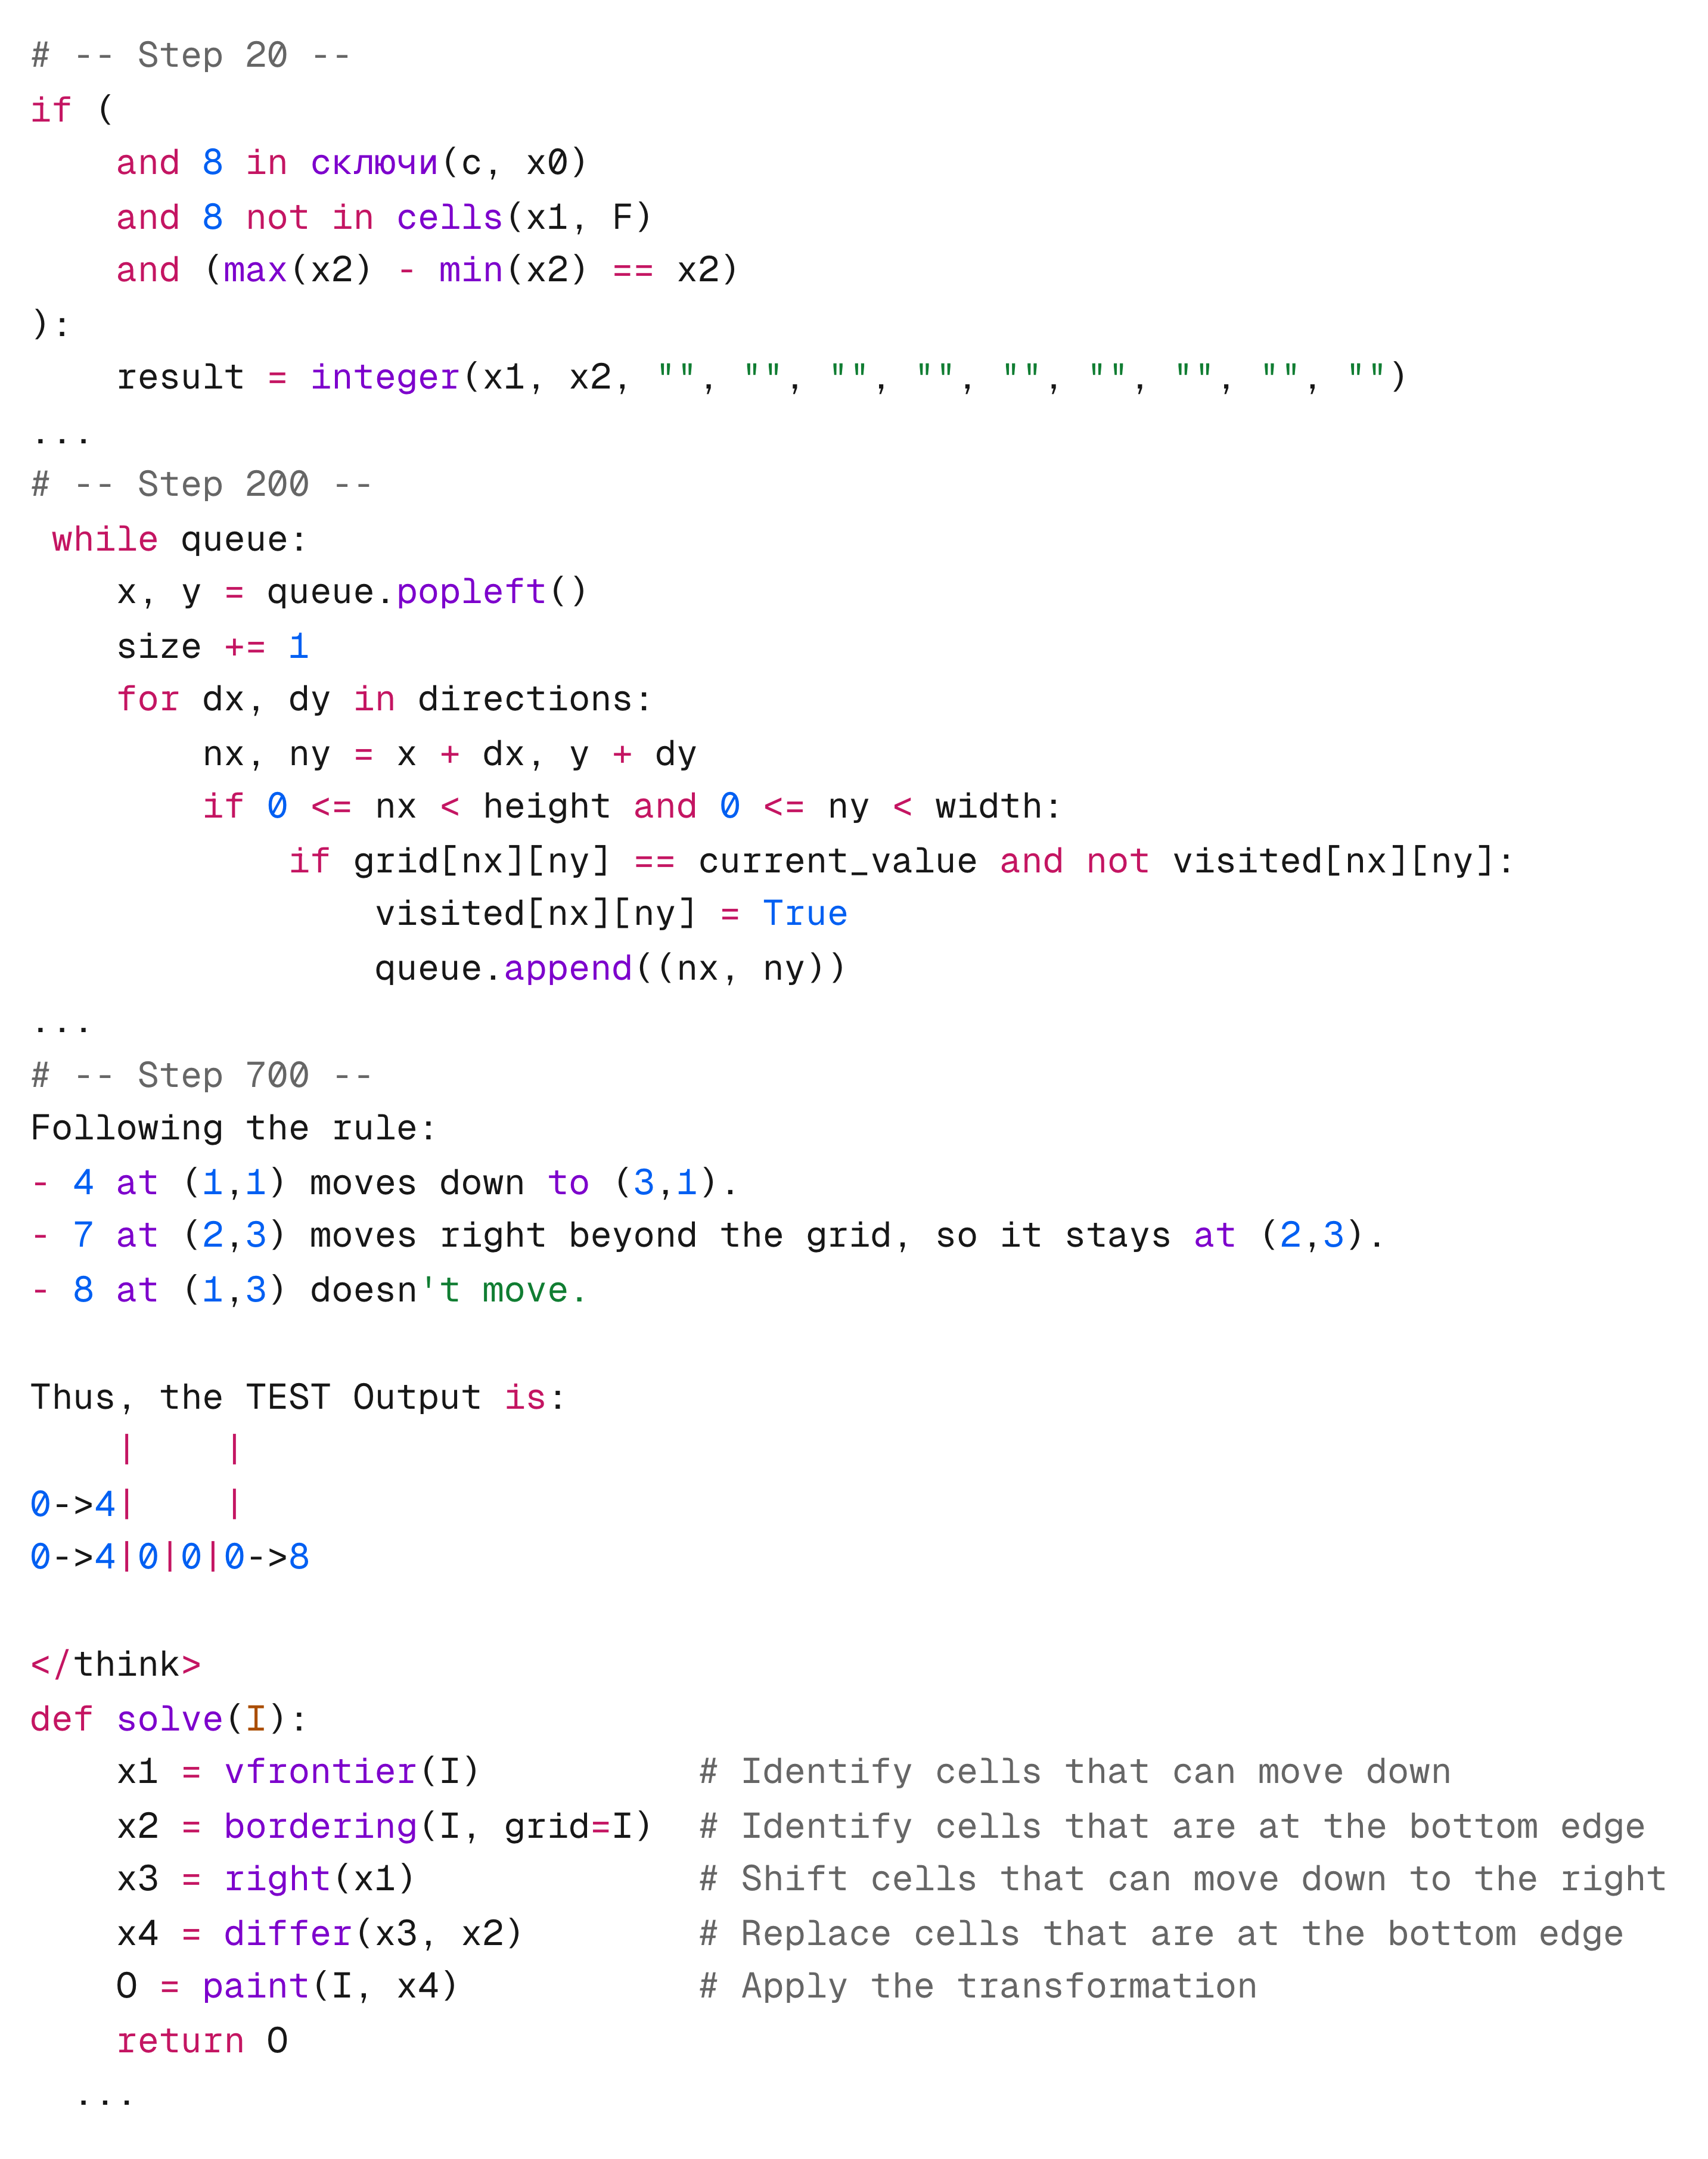
\includegraphics[width=0.95\columnwidth]{bin/codegens.png}
  \caption{Representative samples of generated code over steps.}
  \label{fig:codegens}
\end{figure}


In the literature that trains even larger language models, this low probability of sampling a correct output has been observed by \cite{Greenblatt, Jeremy}. These approaches required thousands of samples before achieving a reasonable chance of selecting the right one. We had hoped this issue would be mitigated over training, but unfortunately, correctness reward signals remained too sparse to provide a reliable signal within each GRPO group.

\subsection{The Purple Rectangle Bias}

During training, we observed an intersting form of cognitive anchoring that emerged from our design of the prompt shared across training steps. We had included a chain-of-thought example, where in a separate puzzle included finding a purple grid to adding colors.

At first, the model paid no heed to our CoT example, but as training progressed, it realized following the CoT helped it solve puzzles correctly, so it decided that hallucinating a purple rectangle would help it enter a correct reasoning mode, where the model would consistently attempt to frame its reasoning through the lens of finding or transforming purple rectangles.

This suggests that hallucination in this context is largely an internal artifact of reasoning steps that are not externally graded. Often, the graded Python output correctly solves the original task. To prevent such biases in the future, we should shuffle our chain-of-thought prompts more frequently to avoid unintended correlations.

\begin{figure}[t]
  \centering
  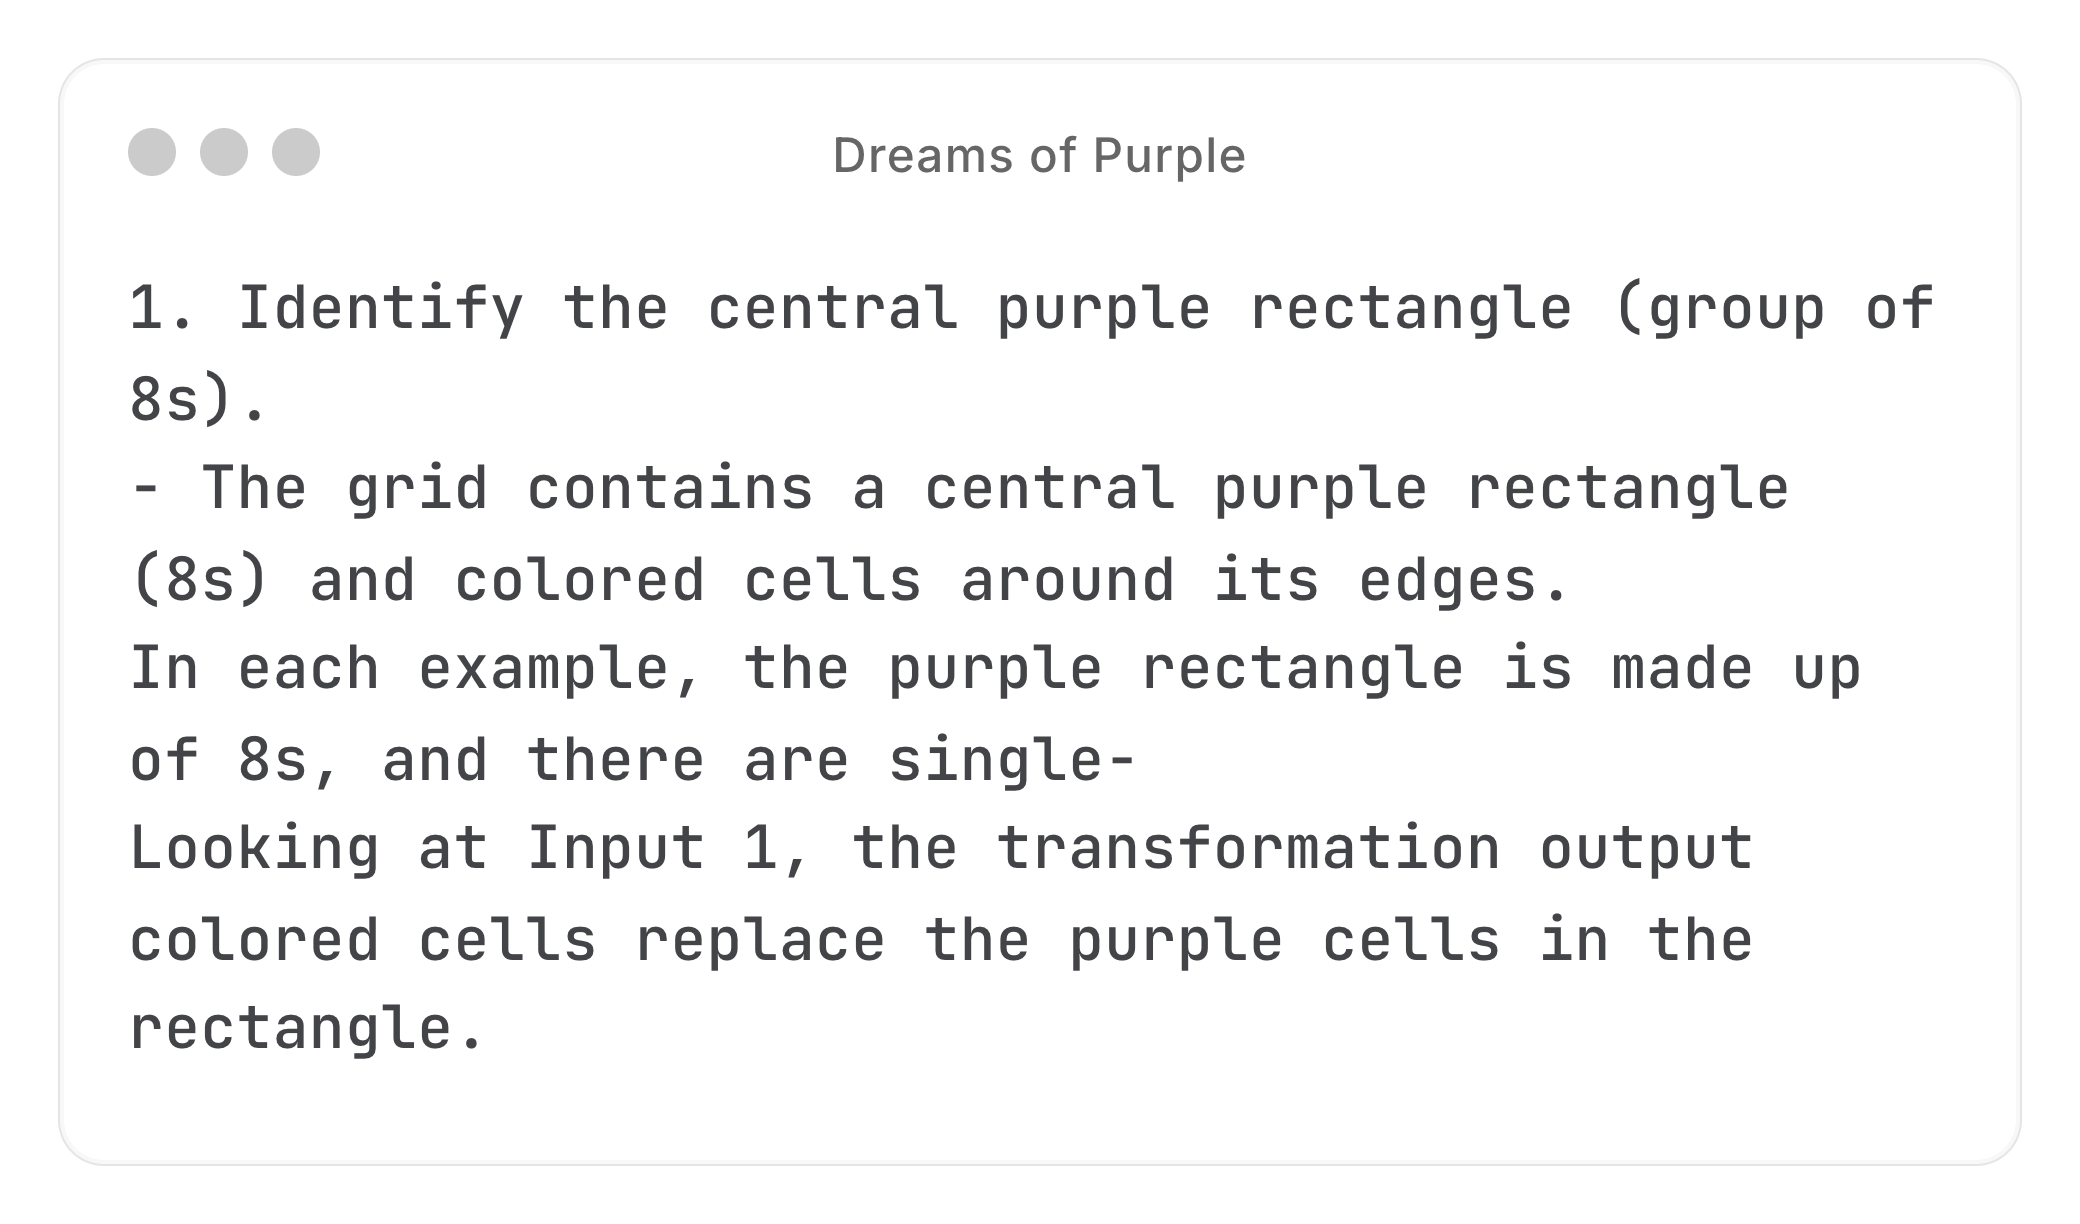
\includegraphics[width=0.95\columnwidth]{bin/purple.png}
  \label{fig:purple}
\end{figure}

\subsection{No 'Aha' Moment}

A key result we observed was that, unlike prior work where models learned to think for longer as training progressed, our model did the opposite. DeepSeek R1-Zero \cite{r1} had an "aha moment," where it realized that using more thinking tokens led to more correct answers without explicit supervision.

However, in our setting—with substantially lower compute—we observed the opposite (Figure \ref{fig:length}). Initially, our model reasoned at length, but as training progressed, it shortened its thinking process significantly. There are two possible explanations for this behavior.

The more forgiving explanation is that the policy learned to "blabber" less. The Qwen model's base reasoning length is derived from distillation fine-tuning on R1 outputs, not RL. Hence it could have learnt to imitate long chains of reasoning well, rather than actual reasoning. We observed this issue in earlier attempts, where one reasoning trace had $k$ distinct thought patterns: the first $(k-1)$ were completely wrong, and only the last was correct. If the RL stage made the model learn that the base behavior was unproductive and that most puzzles followed simpler patterns, it may have naturally converged to shorter reasoning traces.

Indeed, in later iterations, we observed that the model quickly spotted patterns, verified its answers succinctly, and immediately wrote them down without excessive reasoning (Figure \ref{fig:codegens}). This would indicate that it learned to think more efficiently.

A less forgiving explanation is that our style reward was poorly designed. Specifically, we may have overemphasized the importance of correct style while failing to sufficiently reinforce correctness. Since style is much easier to improve than correctness--reflected in our steadily increasing style reward—-it is possible that the model learned to generate correct-looking DSL code quickly without truly engaging in deep reasoning.

If this were the case, we might expect completion length to increase again once style rewards saturate, as the model realizes correctness requires deeper thinking. However, due to compute limitations, we were unable to test this hypothesis further.

\subsection{Variance Reduction}

A major focus of our efforts was on variance reduction. Our initial approaches showed that even large reasoning models (r1, o3) did not provide good sample efficiency, and we could not distill their outputs into our baseline. We speculate that LLMs, in general, struggle with this simple task ARC's abstract reasoning requires framing numbers, colors and letters in a way that is very out-of-pretraining distribution.
\begin{figure}[t]
  \centering
  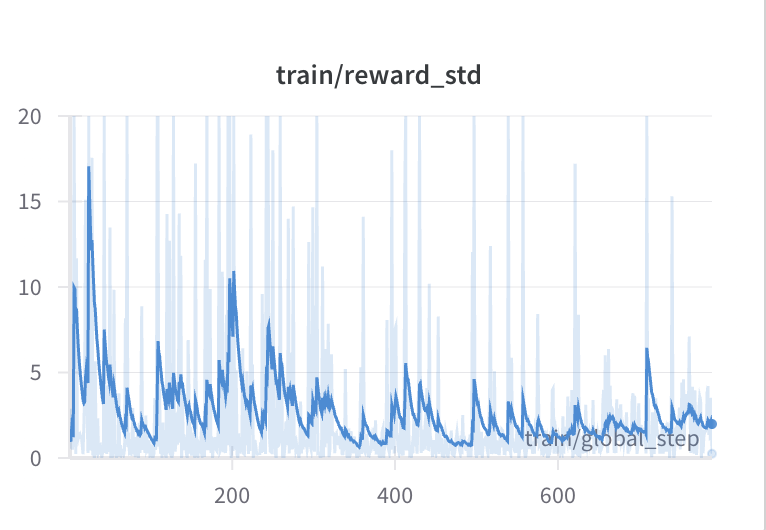
\includegraphics[width=0.95\columnwidth]{bin/rvar.png}
  \caption{stddev of reward within a group $G$, $|G|=4$, over steps.}
  \label{fig:variance}
\end{figure}

Without a reliable baseline, initial training was extremely unstable, and we needed extensive curriculum learning and reward shaping to keep the model on track. However, variance did reduce substantially over training, indicating that the model was slowly converging (Figure \ref{fig:variance}). In our experiment, we primarily focused on solving easier puzzles first, acting as a form of curriculum learning. However, we did not have the compute to fully explore a multi-round approach, where each round would bootstrap the next by leveraging previously trained policies. The many-rounds approach worked well for DeepSeek and may help bootstrap the model toward better reasoning by iteratively increasing task difficulty.

\section{Conclusion}

In summary, we set out to determine whether small models could saturate narrow reasoning tasks like ARC-AGI. We conclude that the reasoning RL recipe still requires more algorithmic and systems improvements to overcome compute-inefficiency, and converge on a low budget.

More broadly, this aligns with observations of ARC designers that even solving ARC-AGI puzzles at scale with reasoning RL remains extremely expensive \cite{Knoop}. Chollet noted that \texttt{o3-high} required roughly \$2,000 per puzzle in test-time compute alone—orders of magnitude more than human problem solvers.

Thus, while AGI may be feasible, it is unlikely to come cheaply to begin with. The next critical step is to develop compute-efficient reinforcement learning techniques that can improve model reasoning in a compute-efficient manner without relying on brute-force search. This includes better curriculum learning, multi-tool RL agents, and methods for guiding models through intermediate steps before solving a full problem.

\bibliography{references}
\bibliographystyle{icml2018}

\appendix
\label{app}

\section{Code Availability}
\label{app:A}
Our training code is available on GitHub \url{https://github.com/photomz/r1-arc}. Our dataset is on HuggingFace: \url{https://huggingface.co/datasets/photonmz/arc_plain}. Our training logs are on Weights \& Biases: \url{https://wandb.ai/photonmz/r1-arc}.


\end{document}

